\documentclass[10pt,onecolumn,a4paper]{article}

\usepackage[a4paper, total={6in, 10in}]{geometry}

\usepackage{graphicx}
\usepackage{url}
\usepackage{amsmath}
\usepackage{listings}

\usepackage[utf8]{inputenc}

\setlength{\parskip}{4pt} % changes vertical space between paragraphs

\begin{document}

	\title{Discovering vulnerabilities in PHP web applications}
	\author{Group no. 23\\Rodrigo Rato - 81500\\Tiago Gonçalves - 81853\\Pedro Correia - 81002}
	\markboth{Software Security - IST Alameda - 1st semester 2017/2018 }{}
	\maketitle



%
%	INTRODUCTION
%
\section{Introduction}

	% \PARstart{}{} creates a tall first letter for this first paragraph
\hspace{3.5mm} Vulnerabilities in PHP code are usually originated from mistakes that programmers make when writing the application code, whether by distraction or unawareness. Sometimes user input isn't handled properly, originating exploitation opportunities like SQL Injection\cite{SQLI} or Cross Site Scripting\cite{XSS}, for example. 

In order to mitigate these risks it is possible to use some analysis tools, which can be of two different kinds - static or dynamic, to make this assessment easier for the developer, which sometimes, doesn't have complete knowledge about the tools he's using or about secure and safe programming.

After analysing the papers proposed for discussion \cite{PROPOSED1}\cite{PROPOSED2}\cite{PROPOSED3}\cite{PROPOSED4}, we proposed to develop a static PHP code analyser inspired by Saner \cite{PROPOSED3}, which compares the inputted PHP file with a given set of patterns, each with a group of entry points, sinks and possible sanitization functions.


%
%	DESIGN AND IMPLEMENTATION
%
\section{Our Design and Implementation}
	\subsection{Design}
	\subsubsection{Prelude}
		\hspace{3.5mm} We decided to adopt an AST based representation using classes like illustrated in the following UML (Unified Modeling Language) class diagram. We will elaborate on this in the following section. 
		\begin{center}
			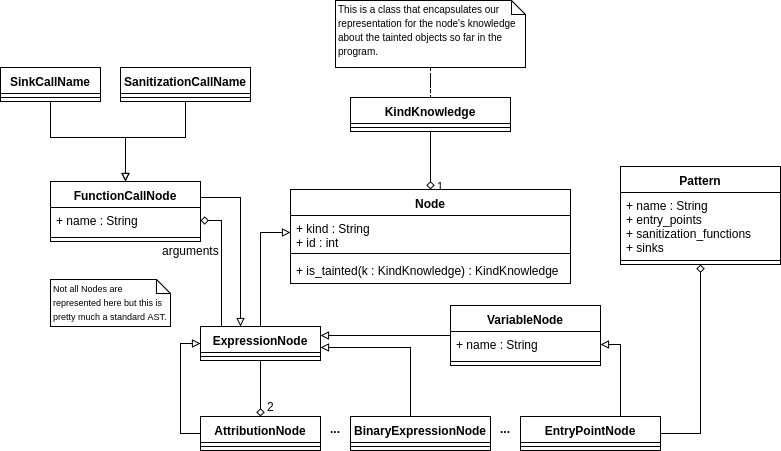
\includegraphics[width=\columnwidth]{uml.png}
		\end{center}
		
	\pagebreak
	\subsubsection{Abstract Syntax Tree}
\hspace{3.5mm} We have designed several classes which represent PHP program nodes and encapsulate the representation that our program receives as input from the Glayzzle PHP Parser demo \cite{PARSERDEMO}.
These classes are structured in a hierarchy according to the context in which they appear in the program in question. 

This means that when we receive a certain PHP program, in the form of JSON (JavaScript Object Notation), we will parse it and instantiate the proper class that we're using to represent that element, taking into account that this element may contain  \emph{sub-elements}.

All nodes have an unique identifier, which will be used to register the associated taint \emph{knowledge} about that node on a custom structure (which is represented by the KindKnowledge class in the diagram above), allowing us to know which patterns are associated to that element. This method is similar to a symbolic table, which is a technique used while compiling a program, but instead of saving the element’s value, it saves it's \emph{taintedness} information.

We have a specific node for \emph{entry points}, \emph{sanitization functions} and \emph{sinks} which are instantiated when one of this elements is detected on the available set of patterns.

When an \emph{entry point} is found, all patterns which have that function name on their \emph{entry points} list are associated to that node.

A \emph{sanitization function} call node obtains the patterns associated to each of the inputted arguments,
if this sanitization node name is referenced in one of those patterns it is removed from the associated pattern list and notifies the user that the argument was sanitized.

A \emph{sink function} call node obtains the patterns associated to each of the inputted arguments, if this \emph{sink function's} name if referenced in one of those patterns, then there is a vulnerability and the user is notified.

In sum, whenever we need to find if a node is tainted or not (and, eventually, by what patterns), each node knows how to evaluate itself, and in case it depends on some children node, it also knows how to delegate that task and handle the resulting knowledge.

		
	\subsubsection{Passing a Node's Knowledge - Information Flow}
\hspace{3.5mm} In the previous section we described how each node delegates the task of finding if it is tainted to it's children, this is possible because we have designed a representation for this knowledge, which is encapsulated by the KindKnowledge class (check UML diagram above). 

This class contains a mapping of a node's unique identifier to a list of patterns associated with that node. Concretely, when an entry point is assigned to a variable, it gets associated to the patterns where this entry point is referenced. If a variable enters a \emph{sanitization function} call which is referenced in the set of patterns mapped by the variable node's unique identifier, then this variable's list of patterns is cleaned accordingly, followed by outputting the sanitization information to the user.
		
If the variable reaches a sink we will then check the set of patterns mapped by this variable node's identifier and, for each pattern, verify is the sink's name is or not referenced, printing out the vulnerability information, if it exists.
		

		
	
	\subsection{Implementation}
		\subsubsection{Input and Output}
\hspace{3.5mm} Our program receives, from the standard input, a path to a text file with the representation of a PHP slice in the form of an AST, represented in JSON using the syntax provided by the Glayzzle PHP Parser \cite{PARSER}.

Therefore, our program is in no way standalone, as we've been converting PHP snippets into their JSON  representation using the Glayzzle PHP Parser demo \cite{PARSERDEMO}.
			
Given a JSON file, with the converted PHP code, in case a certain vulnerability is found, according to the defined vulnerability patterns, a message is printed with the detected vulnerability and the possible sanitization functions to be used.
\pagebreak
\lstinputlisting{output1.txt}

In case a tainted element is sanitized before entering a sink, a message is printed, stating which function sanitized it.
\lstinputlisting{output2.txt}
		
		\subsubsection{Performance}
	
\hspace{3.5mm} In accordance to D. Balzarotti et. al. in Saner\cite{PROPOSED3}, a tool is only useful if it can be run in reasonable time, so that it can be integrated as part of the development process.

According to the previous statement and our presented assumptions, the developed tool runs within reasonable time constraints. Further optimizations could be made in order to optimize our tool, more specifically, related to the way each node element associates the patterns to his taintedness.

Furthermore, a possible optimization would be to refactor classes from the patterns package, as pattern searches can be made more efficient.

		



%
%	GUARANTEES AND SHORTCOMINGS
%
\section{Assurances and shortcomings}
	\subsection{Tool Guarantees}

	\subsection{Tool limitations based on our assumptions}
\subsubsection{Arrays}
\hspace{3.5mm} In case a specific index of an array gets tainted we consider all the array as tainted and not sanitizable at all. This option was taken in order to avoid all elements to be saved in memory. This can generate false positives, since a sanitization function could be applied to all elements of an array, and even so, the previously tainted elements would still be detected as tainted afterwards.

\subsubsection{Cycles}
\hspace{3.5mm} We assume that every loop executes exactly once, in order to avoid infinite loops/recursion or even an incomplete analysis, in case the loop runs a different number of times than what we accounted for, therefore our tool is incomplete. 
It will produce false positives in several cases, such as the one exemplified by slice10.php \cite{SLICES}, where the fourth execution of the loop causes a vulnerability to appear. This vulnerability is not
detected by our tool. 

\subsubsection{Conditions}
\hspace{3.5mm} When faced with a conditional branch, like if and switch, we consider a ‘worst case’ analysis, therefore, if a branch could be taken and that would taint a certain variable, then it is tainted, but even if a branch could sanitize a variable, it would not do it. We also consider that the program always enters the conditional block, maintaining our ‘worst case’ approach. This could present some problems if the program's control flow never enters a conditional branch which sanitizes an element, like in slice15.json \cite{CUSTOMSLICES}. In this case, our approach does not detect a vulnerability, but should, since there is a chance that the conditional block is not taken at all, hence, the element would reach the sink while tainted.

\subsubsection{Function Definitions}
\hspace{3.5mm} Even after designing an approach to this issue we could not complete it's analysis. The tool does not fully implement function definition, further testing and experimentation would be required. A program with a function definition could lead to incoherent results, since entry points, sanitizations and sinks would not be detected if called by a function defined by a programmer.

\subsubsection{Function Calls}
\hspace{3.5mm} As a simplification, we're not considering functions that receive arguments passed by reference. This decision was made in order to safeguard case analysis where a function definition is not present. This renders our analysis incoherent on these specific test cases.

\subsubsection{Expressions}
\hspace{3.5mm} When a variable is handled through string concatenation, or a similar operation, we won't evaluate the resulting expression, as we assume that this case belongs to the domain of dynamic analysis, like verifiable when running slice7.php and slice11.php \cite{SLICES}.  




%
%	CONCLUSION
%
\section{Conclusion}
\hspace{3.5mm}	In this project we have developed a tool that implements a simple way to statically analyse PHP code. After the development process, we concluded that a simple static analysis will always render insufficient results, given the volatility of the relation between user input, the programmer's mindset and the final program behaviour.

The tool that we developed, after some refinements, could be paired with a similar solution, which applies dynamic analysis techniques, to track a wider scope of vulnerabilities, providing a finer grain analysis, thus yielding better results.     
	
\pagebreak

% Now we need a bibliography:
\begin{thebibliography}{5}

	\bibitem{PROPOSED1}
	Yao-Wen Huang, Fang Yu, Christian Hang, Chung-Hung Tsai, D. T. Lee, Sy-Yen Kuo. 
	Securing Web Application Code by Static Analysis and Runtime Protection.
	
	\bibitem{PROPOSED2}
	Gary Wassermann, Zhendong Su. Sound and Precise Analysis of Web Applications
for Injection Vulnerabilities.
	
	\bibitem{PROPOSED3}
	Davide Balzarotti, Marco Cova, Vika Felmetsger, Nenad Jovanovic, Engin Kirda, Christopher Kruegel, and Giovanni Vigna. Saner: Composing Static and Dynamic Analysis to
Validate Sanitization in Web Applications.
	
	\bibitem{PROPOSED4}
	Ibéria Medeiros, Nuno F. Neves, Miguel Correia. Automatic Detection and Correction of Web Application
Vulnerabilities using Data Mining to Predict False Positives.
	

	%Each item starts with a \bibitem{reference} command and the details thereafter.
	\bibitem{XSS} % Transaction paper
	A. Klein. Cross Site Scripting Explained. Technical report,
Sanctum Inc., 2002.

	\bibitem{SQLI}
	C. Anley. Advanced SQL Injection in SQL Server Applications.
Technical report, Next Generation Security Software,
Ltd, 2002.

	\bibitem{WAP} Ibéria Medeiros. Web Application Protection on SourceForge.
	\url{http://awap.sourceforge.net/support.html}
	
	\bibitem{PARSER} Filippo Conti and Ioan Chiriac. Glayzzle PHP Parser.
	\url{https://github.com/glayzzle/php-parser/blob/master/docs/AST.md}
	
	\bibitem{PARSERDEMO} Filippo Conti and Ioan Chiriac. Glayzzle PHP Parser Demo.
	\url{https://glayzzle.com/php-parser/#demo}
	
	\bibitem{SLICES} List of PHP program slices and corresponding JSON representations as provided by the course's teaching faculty.
	
	\bibitem{CUSTOMSLICES} List of PHP program slices and corresponding JSON representations for custom slices that are provided with this project (under proj-slices/custom-slices).
	


\end{thebibliography}

% Your document ends here!
\end{document}
